\title{Survivable Set Connectivity}
\author{
 by Fermi Ma and Erik Waingarten
}
\date{\today}

\documentclass[12pt]{article}
\usepackage{amsmath}
\usepackage{amsthm}
\usepackage{amsfonts}
\usepackage{graphicx}
\usepackage{clrscode4e}

\newtheorem{proposition}{Proposition}
\newtheorem{definition}{Definition}
\newtheorem{lemma}{Lemma}

\begin{document}
\maketitle

\section{Introduction}

In this paper, we analyze the problem of Survivable Set Connectivity (SSC), a generalization of the classical Set Connectivity problem. Set connectivity is formulated as:
\begin{quote}
\textbf{Input}: A graph weighted $G = (V, E)$, $c: E \rightarrow \mathbb{R}$ and a collection of sets $(S_i, T_i)$. \\
\textbf{Output}: A minimum cost subgraph $H \subset G$ such that there is a path between $S_i$ and $T_i$ for each $i$. 
\end{quote}
In SSC, the problem is modified so that each pair of sets $(S_i,T_i)$ must be connected by $k_i$ paths, instead of just 1. More formally, the problem is:

\begin{quote}
\textbf{Input}: A graph weighted $G = (V, E)$, $c: E \rightarrow \mathbb{R}^{\geq 0}$ and a collection of sets $(S_i, T_i)$, along with a value $k$. \\
\textbf{Output}: A minimum cost subgraph $H \subset G$ such that there are $k$ edge-disjoint paths between $S_i$ and $T_i$ for each $i$. 
\end{quote}

Note that this problem generalizes the common connectivity problems. The question of whether there are $k$ connections between $s$ and $t$ sets only one pair $(S_1, T_1)$ where $S_1 = \{ s \}$ and $T_i = \{ t \}$. 

[ GIVE MORE EXAMPLES HERE ]

As with many of these kinds of problems, SSC is $\mathsf{NP}$-hard. The common route taken in 6.856 has been to find polynomial time algorithms for approximations; however, in the case with SSC, it is $\mathsf{NP}$-hard to achieve a polylogarithmic approximation. 

Another possible approach is therefore to relax the question. Instead of requiring at least $k$ edge-disjoint paths, we will allow some sets to have less than $k$ paths, but not too much less. We will present an approximation algorithm which outputs a subgraph of cost $O(polylog(n))$ times the optimum such that for each $(S_i, T_i)$ pairs, there are at least $\Omega(\frac{k}{\log n})$ edge-disjoint paths between $S_i$ and $T_i$. 

The approximation algorithm will follow the usual approach to approximation algorithms of this kind. We will first write the problem as an integer linear program, we solve the linear programming relaxation, and then we round the solution. 

The analysis will be slightly different from the analysis shown in class. Usually, our randomized algorithm will return a feasible solution to the problem, and our analysis work is mostly to bound the cost. This was the case with max-sat, set-cover, and multi-commodity flows. In our case, we will show that the rounded solution will be close to the optimal, but we will work to show that the rounded solution is feasible. 

\section{Linear Programming Formulation}

We can formulate a cut-based integer linear program for SSC. For each edge, we have the variable $x_e$ defined as
\begin{align}
 x_e &= \left\{ \begin{array}{cc} 1 & e \in H \\
                                  0 & \text{ otherwise. } \end{array} \right.
\end{align}
$H$ will be the subgraph consisting of edges $e$ where $x_e = 1$. \\ \\
SSC-LP:
\begin{align}
\min & \sum c(x) x_e  \\
\text{ s.t } & \sum_{e \in \delta(S)} x_e \geq k, \text{ where } S_i \subset S, T_i \subset V - S, \delta(S) \text{ is the edges of the $S$ cut }
\end{align}
This cut-based integer linear program finds exactly $H$. To see why the constraints ensure that each $(S_i, T_i)$ pair has at least $k$ edge disjoint paths, we can look at the cuts corresponding to $S_i$ and $T_i$. First, we let $S = S_i$, then there are $k$ outgoing edges. We can choose to include one more node to $S$, following a particular outgoing edge of the cut in $H$. We can continue doing this until we reach $T_i$. This will trace out a path between $S_i$ and $T_i$. If we do this for each edge, and then we do this for each $(S_i, T_i)$ pair, we can confirm that there are in fact $k$ edge-disjoint paths between each $(S_i, T_i)$ pair. 

There is one caveat that has not been addressed. We have exponentially many constraints! Since there can be exponentially many set $S$ with $S_i \subset S$ and $T_i \subset V - S$. We solve this with a similar idea to semi-definite programming, by giving a separation oracle which runs in polynomial time. 

The separation oracle will just compute the minimum $S_i, T_i$ cut in the graph. What we can do is contract $S_i$ and $T_i$ to single edges, and then compute the min-cut in the remaining graph. If there is a min-cut of size less than $k$, then that cut will correspond to a violating contraint. If the min-cut has size at least $k$, then all cuts have size at least $k$, so we have satisfied the constraints.

The linear programming relaxation to the above program will be the first step of the algorithm. The remaining work will be rounding the fractional solution to an integral solution and satisfy the constraints. 

\section{Tree Embeddings}

The next tool we will need are tree embeddings. We have seen metric embeddings in class. Basically, we had a desired type of object $O$ (in the case of cuts, we had a metric space corresponding to a cut) what we did was come up with a metric space $(X, d)$ and a map $f: (X, d) \rightarrow O$ such that the map satisfied certain properties on the distances. 

Here we will have a similar goal. We want to understand minimum cost weighted graphs, but since analyzing them is hard, we instead study minimum cost weighted trees, and then we map the trees back to the graphs. 

\begin{definition}
A tree embedding of a weighted graph $G = (V, E)$ will be a tree $T = (V_T, E_T)$ with weights $y: E \rightarrow \mathbb{R}^{\geq 0}$ and a function $\text{map} : V_T \cup E_t \rightarrow V \cup P(E)$ ($P(E)$ is the power set of $E$) such that
\begin{align}
\text{map}(V_t) &\subset V \\
\text{map}(E_t) &\subset E
\end{align}
In other words, vertices map to vertices and edges map to edges. We will usually refer to an embedding as $(T, y, \text{map})$. 
\end{definition}

\subsection{Racke Tree Black Box}

We will use a particular type of tree embedding which will allow us to paths in the tree to paths in the graph. 

\begin{definition}
For a given graph $G = (V, E)$, a Racke Tree is a tree embedding of $G$, $(T, y, \text{map})$ such that:
\begin{enumerate}
\item $\text{map}$ restricted to the leafs of $T$ is a bijection with the vertices of $G$.
\item For each edge $e \in E_t$ joining $u$ and $v$, $\text{map}(e)$ is a path joining nodes $\text{map}(u)$ and $\text{map}(v)$.
\item For some edge $e \in E_t$, $y_e$ (the cost of the edge) is a special quantity. Removing $y_e$ cuts the tree into two components, and so the leaves in the two components form a cut $\delta(S)$. Figure~\ref{fig:rackecut} gives an example for one such cut induced by an edge.
\begin{align}
y_e &= \sum_{e' \in \delta(S)} x_e
\end{align}
\end{enumerate}
\end{definition}

\begin{figure}
\centering
\label{fig:rackecut}
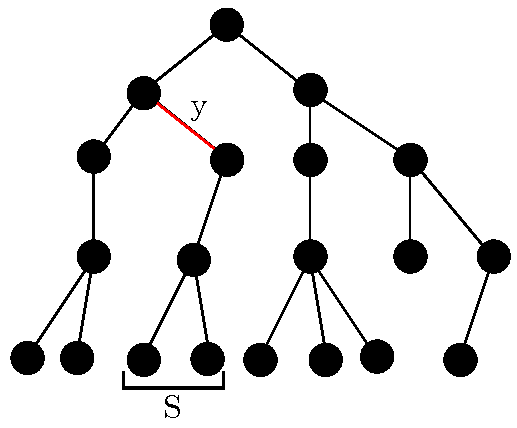
\includegraphics[width=0.5\linewidth]{Rackecut.pdf}
\caption{Racke tree cut induced by an edge in the tree.}
\end{figure}

Having made these definition, we can refer to the inverse $\text{map}^{-1}$ in the obvious manner. $\text{map}^{-1}$ on a vertex will map to the corresponding leaf, and $\text{map}^{-1}$ on an edge in the graph will map to all edges in the tree whose paths contain that edge. 

\begin{definition}
Given a Racke tree, the load on an edge of the graph $e \in E$ is
\begin{align}
load(e) &= \sum_{f \in \text{map}^{-1}(e)} y_f
\end{align}
The relative load, $rload(e) = \dfrac{load(e)}{x_e}$. 
\end{definition}

Figure~\ref{fig:racketree} gives an example of a Racke tree with the mapping. Each red vertex of the tree is mapped to another red vertex on the graph, and the edge between them corresponds to a path between the red vertices. This gives us a simple way to map flows from Racke trees to the graph and vice-versa. 

In particular, if we have a multicommodity flow $\{ f_i \}$ on the graph, then we can easily map into a multicommodity flow on the Racke tree. If there is a flow $f_i$ from $s_i$ to $t_i$, then we find leaves $s_i^{T}=\text{map}^{-1}(s_i)$ and $t_i^T\text{map}^{-1}(t_i)$ and route $f_i$ units of flow through the unique path from $s_i$ to $t_i$.

For obtaining a flow on the graph given one on the Racke tree, if $f_i^T(e)$ is the flow of commodity $i$ on the tree on $e \in E_t$, then we route $f_i^T(e)$ units of flow down the path given by $\text{map}(e)$.   

\begin{figure}
\label{fig:racketree}
\centering
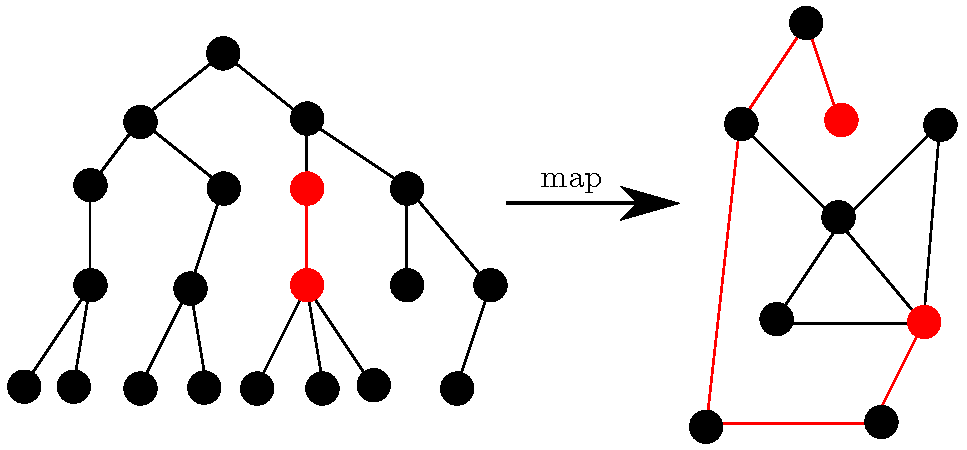
\includegraphics[width=\linewidth]{Rackeembeddinggraph.pdf}
\caption{Example Racke Tree where red nodes are mapped and edge maps to a path.}
\end{figure}

There are some crucial properties of Racke trees which we will treat as black boxes. We will define these as lemmas without proof, and we refer to [CITE] for the proofs.

\begin{lemma}
\label{lem:mapflows}
If we have a graph $G = (V, E)$ and capacities $x: E \rightarrow \mathbb{R}^{\geq 0}$ and a Racke tree $(T, y, \text{map})$. A multicommodity flow on $G$, $\{ f_i \}$, maps directly to a multicommodity flow on the tree which is also feasible. Likewise, a multicommodity flow on $T$ maps directly into a multicommodity flow on the graph, with the small caveat that we must multiply the capacity of the edge by the relative load. 
\end{lemma}

\begin{lemma}
\label{lem:rload}
For some given graph $G = (V, E)$ and capacities $x: E \rightarrow \mathbb{R}^{\geq 0}$, we can sample efficiently from Racke trees of $G$, such that 
\begin{align}
\max_{e \in E} \textbf{E}[rload(e)] &\leq \alpha = O(\log n) 
\end{align}
\end{lemma}

\begin{lemma}
\label{thm:height}
The height of the trees sampled is $O(\log nC)$, where $C$ is the ratio of the largest to smallest capacity in $G$. In our cases, the height will always be $O(\log n)$. 
\end{lemma}

\subsection{RoundGKR Black Box}

The RoundGKR algorithm is an algorithm to rounding algorithm used for the Group Steiner Tree problem. We first describe the problem and give the algorithm. \\

Group Steiner Tree:
\begin{quote}
\textbf{Input}: A rooted tree $T = (V_t, E_t)$ at $r$ with costs $c: E_t \rightarrow \mathbb{R}^{\geq 0}$ as well as subsets of vertices $\{ T_i \}$. \\
\textbf{Output}: A minimum cost subtree $H \subset T$ with a path from $r$ to $t_i$ for some $t \in T_i$ for all $i$.
\end{quote}

A similar linear program produces a fractional solution, and the algorith RoundGKR is a way of rounding the solution back. The optimum to the linear program will be a set of values for each edge $y_e \in [0, 1]$. Since we are in a tree setting and we are looking for paths from the root, we can assume that $y_{p(e)} \geq y_e$ (parent edges are always greater).

The RoundGKR is simple, it starts at the root and makes its way down the tree as its being built. It includes the edge $e$ in the subtree with probability $\frac{y_e}{y_{p(e)}}$. A simple inductive argment shows that an edge $e$ is chosen with probability $y_e$. This is because $Pr[\text{include $e$}] = Pr[\text{include $e$ $|$ include $p(e)$}]*Pr[\text{include $p(e)$}] = y_e$ (if we don't include $p(e)$, then we don't include $e$. 

The important property of the algorithm can be summarized in the following lemma, whose proof we refer to [CITE].

\begin{lemma}
\label{lem:findpath}
Suppose that $T = (V_t, E_t)$ support a flow of at least $1$ from $T_i$ to the root $r$ without the edges $F_t$. Then the RoundGKR returns a solution with a path in $T$ from $T_i$ to $r$ without using $F_t$ with probability at least $\Omega(\frac{1}{\log n})$. 
\end{lemma}

We will rely on this lemma heavily. In fact, since we need $\Omega(\frac{k}{\log n})$ edge-disjoint paths, we will argue that if we let $F_t$ be any set of at most $\Omega(\frac{k}{\log n})$ edges, then we still have a path, and therefore, we have $\Omega(\frac{k}{\log n})$ paths.  

\section{Algorithm}

Now we will combine the ideas of the linear program to approximate the survival set connectivity. We copy the algorithm as it is written in the paper below, although we will separate the algorithm into portions and explain each portion in detail.
\begin{codebox}
\li Set $H \leftarrow \emptyset$
\li Compute linear program SSC-LP and set to zero any $x_e < \dfrac{k}{n^2}$.
\li Let $x' \leftarrow x*\frac{4}{k}$. 
\li Prepare $\mathcal{D}$ be the distribution of Racke tree embeddings for $G$ with $x'$.
\li \For $\tau$ rounds \Do
\li Sample $(T, y, \text{map})$ from $\mathcal{D}$. 
\li \For $q = 0, ..., 2\log n$ \Do
\li \For $v \in V_t$ \Do
\li With probability $\min\{1, \dfrac{4}{2^q}\}$, $q$-mark $v$
\li \If $v$ is $q$-marked \Then
\li Set $y^{v, q}\leftarrow 2^{q+1}y$ and $E^{v,q} \leftarrow \emptyset$.
\li \For $\tau'$ iterations, \Do
\li $E^{v,q} \leftarrow E^{v,q} \cup$ RoundGKR$(T_v, v, y^{v,q})$ \End
\li $H \leftarrow H \cup \text{map}(E^{v,q})$ \End \End \End \End
\li return $H$
\end{codebox}

In order to understand the ideas of the algorithm, it is important to understand the ideas of the analysis. We summarize the ideas of the analysis here:
\begin{enumerate}
\item Set a particular set of edges $F$ of size at most $\Omega(\dfrac{k}{\log n})$. 
\item Argue that with probability at most $\frac{1}{2}$, the edges in $F$ are not necessary for connectivity by claiming that the total $load$ on the edges in low. 
\item We will condition on this probability to show that if we remove $\text{map}(F)$ on the tree, we still have sufficient flow from each $s_i$ to $t_i$. This flow must go up the tree to some common ancestor $v$ and then back down.
\item Then we will claim that at some $v$, it gets marked and the RoundGKR algorithm which is rooted at $v$ finds the two paths from $v$ to $s_i$ and $t_i$, and so the path will be included with sufficient probability and exclude $F$.
\item We finally union bound over all $F$ and over all $i$ to show that we succeed with constant probability. 
\end{enumerate}

\subsection{Analysis}

It is straight forward to show that the cost is not too bad.

\begin{lemma}
$\textbf{E}[c(H)] = O(\log^4n(\frac{\log h}{k}+1)) * c(x)$, where $c(x) = \sum_e c(e)x_e$. 
\end{lemma}
This shows that if the algorithm has $\Omega(\frac{k}{\log n})$ edge-disjoint paths between each $(S_i, T_i)$ pair, then it is a polylogarithmic approximation. 

\begin{proof}
The proof follows the common strategy: we bound the probability that a given edge is included. If the probabability that a given edge is included is bounded by $O(\log^4n(\frac{\log h}{k} + 1))x_e$, then by linearity of expectation, we would show the claim.

Let $(T = (V_t, E_t), y, \text{map})$ be a Racke tree sampled from $\mathcal{D}$. By line $12$ of the algorithm, for an edge $e \in H$, there needs to be some $e' \in E_t$ such that $e \in \text{map}(e')$ and $e' \in E^{v,q}$ for some $v \in V_t$ and $q$. In addition, $v$ needed to have been $q$-marked. 

For each $q$ and $v$, $v$ is $q$-marked with probability at most $\frac{4}{2^{-q}}$. In any of the $\tau'$ iterations of the RoundGKR algorithm where $v$ was $q$-marked, an edge is selected with probability $2^{q+1}y_e$. 

Since a given edge has $height(T)$ ancestors, it will take part in $height(T)$ possible $v$'s which can be $q$-marked. So the probability that an edge $e$ is included is at most 
\begin{align}
height(T) \sum_q \frac{4}{2^{-q}} 2^{q+1} y_e \tau' &= height(T) \tau' y_2 \sum_q 2 \\
&= O(\log^3 n) y_e 
\end{align}
This is because $height(T) = O(\log n)$, $\tau' = O(\log n)$, and $q$ takes $O(\log n)$ possible values.

So we have shown that the probability that a given edge is included in a particular sampling of a Racke tree is $O(\log^3 n) y_e$. 
 
\end{proof}

\section{Conclusion}

\subsection{Open Problems}

\end{document}